\chapter{Consultas en rangos}

\index{consultas en rangos}
\index{consultas de suma}
\index{consultas de mínimo}
\index{consultas de máximo}

En este capítulo discutiremos estructuras de datos
que nos permiten procesar consultas en rangos (\textit{range queries})
de manera eficiente. En una \key{consulta en rango},
nuestra tarea es calcular un valor
basado en un subarreglo de un arreglo.
Las consultas típicas son:
\begin{itemize}
    \item $\texttt{suma}_q(a,b)$: calcular la suma de valores en el rango $[a,b]$
    \item $\texttt{min}_q(a,b)$: encontrar el valor mínimo en el rango $[a,b]$
    \item $\texttt{max}_q(a,b)$: encontrar el valor máximo en el rango $[a,b]$
\end{itemize}

Donde la letra \textit{q} denota una consulta en el subarreglo. Por ejemplo, considera el rango $[3,6]$ en el siguiente arreglo:
\begin{center}
    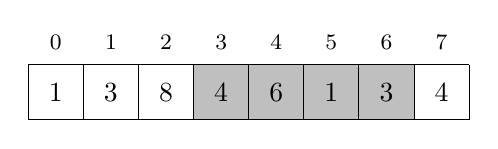
\begin{tikzpicture}[scale=0.7]
        \fill[color=lightgray] (3,0) rectangle (7,1);
        \draw (0,0) grid (8,1);

        \node at (0.5,0.5) {$1$};
        \node at (1.5,0.5) {$3$};
        \node at (2.5,0.5) {$8$};
        \node at (3.5,0.5) {$4$};
        \node at (4.5,0.5) {$6$};
        \node at (5.5,0.5) {$1$};
        \node at (6.5,0.5) {$3$};
        \node at (7.5,0.5) {$4$};

        \footnotesize
        \node at (0.5,1.4) {$0$};
        \node at (1.5,1.4) {$1$};
        \node at (2.5,1.4) {$2$};
        \node at (3.5,1.4) {$3$};
        \node at (4.5,1.4) {$4$};
        \node at (5.5,1.4) {$5$};
        \node at (6.5,1.4) {$6$};
        \node at (7.5,1.4) {$7$};
    \end{tikzpicture}
\end{center}
En este caso, $\texttt{suma}_q(3,6)=14$,
$\texttt{min}_q(3,6)=1$ y $\texttt{max}_q(3,6)=6$.

Una forma simple de procesar consultas de rango es usar
un bucle que recorre todos los valores del arreglo en el rango.
Por ejemplo, podemos usar la siguiente función para procesar
consultas de suma en un arreglo:

\begin{lstlisting}
int sum(int a, int b) {
    int s = 0;
    for (int i = a; i <= b; i++) {
        s += arreglo[i];
    }
    return s;
}
\end{lstlisting}

Esta función funciona en $O(n)$,
donde $n$ es el tamaño del arreglo.
Por lo tanto, podemos procesar $q$ consultas en $O(nq)$
usando la función.
Sin embargo, si tanto $n$ como $q$ son grandes, este método
es muy lento. Afortunadamente, resulta que existen
maneras de procesar consultas de rango mucho más eficientemente.

\section{Consultas en arreglos estáticos}

Primero nos enfocaremos en una situación donde
el arreglo es \emph{estático}, es decir,
los valores del arreglo nunca se actualizan entre las consultas.
En este caso, basta con construir
una estructura de datos estática que nos indique
la respuesta para cualquier consulta posible.

\subsubsection{Consultas de suma}

\index{arreglo de sumas de prefijos}

Podemos fácilmente procesar consultas de suma en un arreglo estático
construyendo un \key{arreglo de sumas de prefijos}.
Cada valor en este arreglo equivale a la suma de valores en el
arreglo original \emph{hasta} esa posición, o sea, el valor en
cada posición $k$ es igual a $\texttt{suma}_q(0,k)$.
El arreglo de sumas de prefijos puede construirse en $O(n)$,
ya que cada valor solo depende del anterior.

Por ejemplo, considera el siguiente arreglo:

\begin{center}
    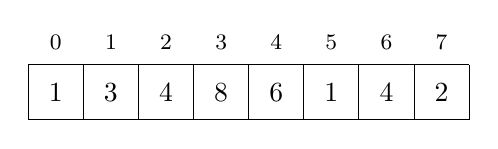
\begin{tikzpicture}[scale=0.7]
        %\fill[color=lightgray] (3,0) rectangle (7,1);
        \draw (0,0) grid (8,1);

        \node at (0.5,0.5) {$1$};
        \node at (1.5,0.5) {$3$};
        \node at (2.5,0.5) {$4$};
        \node at (3.5,0.5) {$8$};
        \node at (4.5,0.5) {$6$};
        \node at (5.5,0.5) {$1$};
        \node at (6.5,0.5) {$4$};
        \node at (7.5,0.5) {$2$};

        \footnotesize
        \node at (0.5,1.4) {$0$};
        \node at (1.5,1.4) {$1$};
        \node at (2.5,1.4) {$2$};
        \node at (3.5,1.4) {$3$};
        \node at (4.5,1.4) {$4$};
        \node at (5.5,1.4) {$5$};
        \node at (6.5,1.4) {$6$};
        \node at (7.5,1.4) {$7$};
    \end{tikzpicture}
\end{center}

Su arreglo de sumas de prefijos es el siguiente:
\begin{center}
    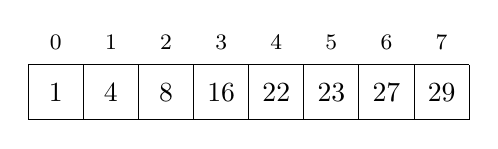
\begin{tikzpicture}[scale=0.7]
        \draw (0,0) grid (8,1);

        \node at (0.5,0.5) {$1$};
        \node at (1.5,0.5) {$4$};
        \node at (2.5,0.5) {$8$};
        \node at (3.5,0.5) {$16$};
        \node at (4.5,0.5) {$22$};
        \node at (5.5,0.5) {$23$};
        \node at (6.5,0.5) {$27$};
        \node at (7.5,0.5) {$29$};

        \footnotesize
        \node at (0.5,1.4) {$0$};
        \node at (1.5,1.4) {$1$};
        \node at (2.5,1.4) {$2$};
        \node at (3.5,1.4) {$3$};
        \node at (4.5,1.4) {$4$};
        \node at (5.5,1.4) {$5$};
        \node at (6.5,1.4) {$6$};
        \node at (7.5,1.4) {$7$};
    \end{tikzpicture}
\end{center}

Dado que el arreglo de sumas de prefijos contiene todo valor
de $\texttt{suma}_q(0,k)$,
podemos calcular cualquier valor de
$\texttt{suma}_q(a,b)$ en $O(1)$ de la siguiente manera:
\[ \texttt{suma}_q(a,b) = \texttt{suma}_q(0,b) - \texttt{suma}_q(0,a-1)\]
Definiendo $\texttt{suma}_q(0,-1)=0$,
la fórmula anterior también se cumple cuando $a=0$.

Por ejemplo, considera el rango $[3,6]$:
\begin{center}
    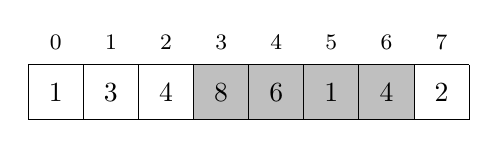
\begin{tikzpicture}[scale=0.7]
        \fill[color=lightgray] (3,0) rectangle (7,1);
        \draw (0,0) grid (8,1);

        \node at (0.5,0.5) {$1$};
        \node at (1.5,0.5) {$3$};
        \node at (2.5,0.5) {$4$};
        \node at (3.5,0.5) {$8$};
        \node at (4.5,0.5) {$6$};
        \node at (5.5,0.5) {$1$};
        \node at (6.5,0.5) {$4$};
        \node at (7.5,0.5) {$2$};

        \footnotesize
        \node at (0.5,1.4) {$0$};
        \node at (1.5,1.4) {$1$};
        \node at (2.5,1.4) {$2$};
        \node at (3.5,1.4) {$3$};
        \node at (4.5,1.4) {$4$};
        \node at (5.5,1.4) {$5$};
        \node at (6.5,1.4) {$6$};
        \node at (7.5,1.4) {$7$};
    \end{tikzpicture}
\end{center}

En este caso $\texttt{suma}_q(3,6)=8+6+1+4=19$.
Esta suma se puede calcular a partir de
dos valores del arreglo de suma de prefijos:
\begin{center}
    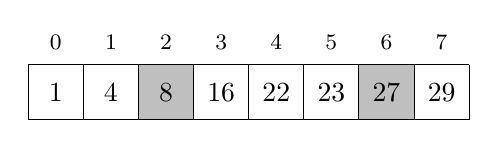
\begin{tikzpicture}[scale=0.7]
        \fill[color=lightgray] (2,0) rectangle (3,1);
        \fill[color=lightgray] (6,0) rectangle (7,1);
        \draw (0,0) grid (8,1);

        \node at (0.5,0.5) {$1$};
        \node at (1.5,0.5) {$4$};
        \node at (2.5,0.5) {$8$};
        \node at (3.5,0.5) {$16$};
        \node at (4.5,0.5) {$22$};
        \node at (5.5,0.5) {$23$};
        \node at (6.5,0.5) {$27$};
        \node at (7.5,0.5) {$29$};

        \footnotesize
        \node at (0.5,1.4) {$0$};
        \node at (1.5,1.4) {$1$};
        \node at (2.5,1.4) {$2$};
        \node at (3.5,1.4) {$3$};
        \node at (4.5,1.4) {$4$};
        \node at (5.5,1.4) {$5$};
        \node at (6.5,1.4) {$6$};
        \node at (7.5,1.4) {$7$};
    \end{tikzpicture}
\end{center}
Así, $\texttt{suma}_q(3,6)=\texttt{suma}_q(0,6)-\texttt{suma}_q(0,2)=27-8=19$.

También es posible generalizar esta idea
a dimensiones superiores.
Por ejemplo, podemos construir una matriz
de sumas de prefijos que se puede utilizar para calcular
la suma de cualquier subarreglo rectangular en $O(1)$.
Cada suma en dicho arreglo corresponde a
un subarreglo que comienza en la esquina superior
izquierda del arreglo.

\pagebreak
La siguiente imagen ilustra la idea:
\begin{center}
    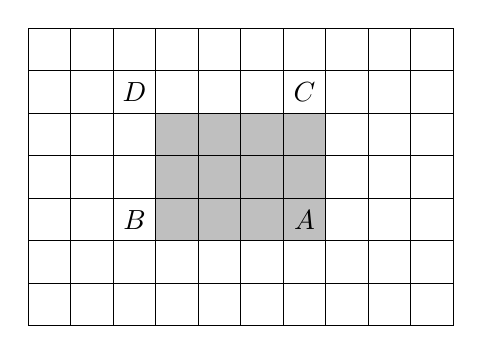
\begin{tikzpicture}[scale=0.54]
        \draw[fill=lightgray] (3,2) rectangle (7,5);
        \draw (0,0) grid (10,7);
        \node[anchor=center] at (6.5, 2.5) {$A$};
        \node[anchor=center] at (2.5, 2.5) {$B$};
        \node[anchor=center] at (6.5, 5.5) {$C$};
        \node[anchor=center] at (2.5, 5.5) {$D$};
    \end{tikzpicture}
\end{center}

La suma del subarreglo gris se puede calcular
usando la fórmula
\[S(A) - S(B) - S(C) + S(D),\]
donde $S(X)$ denota la suma de valores
en un subarreglo rectangular
desde la esquina superior izquierda
hasta la posición de $X$.

\subsubsection{Consultas de mínimo}

\index{tabla dispersa}

Las consultas de mínimo son más difíciles de procesar
que las consultas de suma.
Sin embargo, hay un método de preprocesamiento bastante simple
en $O(n \log n)$ luego del cual podemos responder a
cualquier consulta de mínimo en $O(1)$.\footnote{Esta técnica
    fue introducida en \cite{ben00} y a veces
    se llama método de \key{tabla dispersa} (\textit{sparse table}).
    También existen técnicas más sofisticadas \cite{fis06} donde
    el tiempo de preprocesamiento es solo $O(n)$, pero tales algoritmos
    no son necesarios en programación competitiva.}
Ten en cuenta que, dado que las consultas de mínimo y máximo se pueden
procesar de manera similar, nos centraremos en las consultas de mínimo.

La idea es precalcular todos los valores de
$\textrm{min}_q(a,b)$ donde
$b-a+1$ (la longitud del rango $[a,b]$) sea una potencia de dos.
Por ejemplo, para el arreglo

\begin{center}
    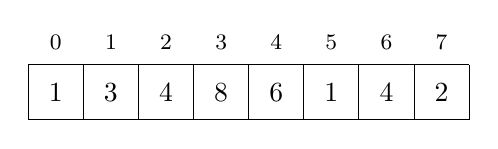
\begin{tikzpicture}[scale=0.7]
        \draw (0,0) grid (8,1);

        \node at (0.5,0.5) {$1$};
        \node at (1.5,0.5) {$3$};
        \node at (2.5,0.5) {$4$};
        \node at (3.5,0.5) {$8$};
        \node at (4.5,0.5) {$6$};
        \node at (5.5,0.5) {$1$};
        \node at (6.5,0.5) {$4$};
        \node at (7.5,0.5) {$2$};

        \footnotesize
        \node at (0.5,1.4) {$0$};
        \node at (1.5,1.4) {$1$};
        \node at (2.5,1.4) {$2$};
        \node at (3.5,1.4) {$3$};
        \node at (4.5,1.4) {$4$};
        \node at (5.5,1.4) {$5$};
        \node at (6.5,1.4) {$6$};
        \node at (7.5,1.4) {$7$};
    \end{tikzpicture}
\end{center}
se calculan los siguientes valores:

\begin{center}
    \begin{tabular}{ccc}

        \begin{tabular}{lll}
            $a$ & $b$ & $\texttt{min}_q(a,b)$ \\
            \hline
            0   & 0   & 1                     \\
            1   & 1   & 3                     \\
            2   & 2   & 4                     \\
            3   & 3   & 8                     \\
            4   & 4   & 6                     \\
            5   & 5   & 1                     \\
            6   & 6   & 4                     \\
            7   & 7   & 2                     \\
        \end{tabular}

         &

        \begin{tabular}{lll}
            $a$ & $b$ & $\texttt{min}_q(a,b)$ \\
            \hline
            0   & 1   & 1                     \\
            1   & 2   & 3                     \\
            2   & 3   & 4                     \\
            3   & 4   & 6                     \\
            4   & 5   & 1                     \\
            5   & 6   & 1                     \\
            6   & 7   & 2                     \\
            \\
        \end{tabular}

         &

        \begin{tabular}{lll}
            $a$ & $b$ & $\texttt{min}_q(a,b)$ \\
            \hline
            0   & 3   & 1                     \\
            1   & 4   & 3                     \\
            2   & 5   & 1                     \\
            3   & 6   & 1                     \\
            4   & 7   & 1                     \\
            0   & 7   & 1                     \\
            \\
            \\
        \end{tabular}
    \end{tabular}
\end{center}

El número de valores precalculados es $O(n \log n)$,
porque hay $O(\log n)$ longitudes de rango
que son potencias de dos.
Los valores se pueden calcular de manera eficiente
usando la fórmula recursiva
\[\texttt{min}_q(a,b) = \min(\texttt{min}_q(a,a+w-1),\texttt{min}_q(a+w,b)),\]
donde $b-a+1$ es una potencia de dos y $w=(b-a+1)/2$.
Calcular todos esos valores toma un tiempo de $O(n \log n)$.

Después de esto, cualquier valor de $\texttt{min}_q(a,b)$ se puede calcular
en  $O(1)$ como el mínimo de dos valores precalculados.
Sea $k$ la mayor potencia de dos que no exceda $b-a+1$.
Podemos calcular el valor de $\texttt{min}_q(a,b)$ usando la fórmula
\[\texttt{min}_q(a,b) = \min(\texttt{min}_q(a,a+k-1),\texttt{min}_q(b-k+1,b)).\]
En la fórmula anterior, el rango $[a,b]$ se representa
como la unión de los rangos $[a,a+k-1]$ y $[b-k+1,b]$, ambos de longitud $k$.

Como ejemplo, considera el rango $[1,6]$:
\begin{center}
    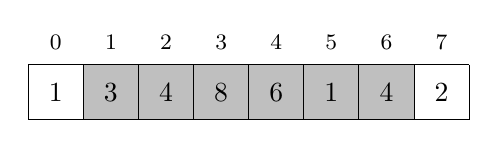
\begin{tikzpicture}[scale=0.7]
        \fill[color=lightgray] (1,0) rectangle (7,1);
        \draw (0,0) grid (8,1);

        \node at (0.5,0.5) {$1$};
        \node at (1.5,0.5) {$3$};
        \node at (2.5,0.5) {$4$};
        \node at (3.5,0.5) {$8$};
        \node at (4.5,0.5) {$6$};
        \node at (5.5,0.5) {$1$};
        \node at (6.5,0.5) {$4$};
        \node at (7.5,0.5) {$2$};

        \footnotesize
        \node at (0.5,1.4) {$0$};
        \node at (1.5,1.4) {$1$};
        \node at (2.5,1.4) {$2$};
        \node at (3.5,1.4) {$3$};
        \node at (4.5,1.4) {$4$};
        \node at (5.5,1.4) {$5$};
        \node at (6.5,1.4) {$6$};
        \node at (7.5,1.4) {$7$};
    \end{tikzpicture}
\end{center}
La longitud del rango es 6,
y la mayor potencia de dos que no
exceda 6 es 4.
Por lo tanto, el rango $[1,6]$ es
la unión de los rangos $[1,4]$ y $[3,6]$:
\begin{center}
    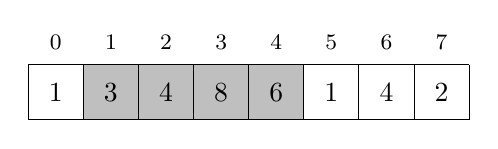
\begin{tikzpicture}[scale=0.7]
        \fill[color=lightgray] (1,0) rectangle (5,1);
        \draw (0,0) grid (8,1);

        \node at (0.5,0.5) {$1$};
        \node at (1.5,0.5) {$3$};
        \node at (2.5,0.5) {$4$};
        \node at (3.5,0.5) {$8$};
        \node at (4.5,0.5) {$6$};
        \node at (5.5,0.5) {$1$};
        \node at (6.5,0.5) {$4$};
        \node at (7.5,0.5) {$2$};

        \footnotesize
        \node at (0.5,1.4) {$0$};
        \node at (1.5,1.4) {$1$};
        \node at (2.5,1.4) {$2$};
        \node at (3.5,1.4) {$3$};
        \node at (4.5,1.4) {$4$};
        \node at (5.5,1.4) {$5$};
        \node at (6.5,1.4) {$6$};
        \node at (7.5,1.4) {$7$};
    \end{tikzpicture}
\end{center}
\begin{center}
    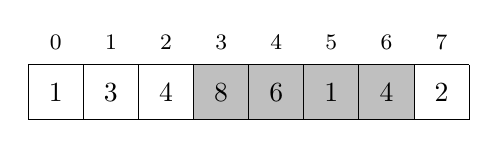
\begin{tikzpicture}[scale=0.7]
        \fill[color=lightgray] (3,0) rectangle (7,1);
        \draw (0,0) grid (8,1);

        \node at (0.5,0.5) {$1$};
        \node at (1.5,0.5) {$3$};
        \node at (2.5,0.5) {$4$};
        \node at (3.5,0.5) {$8$};
        \node at (4.5,0.5) {$6$};
        \node at (5.5,0.5) {$1$};
        \node at (6.5,0.5) {$4$};
        \node at (7.5,0.5) {$2$};


        \footnotesize
        \node at (0.5,1.4) {$0$};
        \node at (1.5,1.4) {$1$};
        \node at (2.5,1.4) {$2$};
        \node at (3.5,1.4) {$3$};
        \node at (4.5,1.4) {$4$};
        \node at (5.5,1.4) {$5$};
        \node at (6.5,1.4) {$6$};
        \node at (7.5,1.4) {$7$};
    \end{tikzpicture}
\end{center}
Dado que $\texttt{min}_q(1,4)=3$ y $\texttt{min}_q(3,6)=1$,
concluimos que $\texttt{min}_q(1,6)=1$.


\section{Árbol binario indexado}

\index{árbol binario indexado}
\index{árbol de Fenwick}

Un \key{árbol binario indexado} o un \key{árbol de Fenwick}\footnote{La
    estructura del árbol binario indexado fue presentada por P. M. Fenwick en 1994 \cite{fen94}.}
puede verse como una variante dinámica del arreglo de sumas de prefijos.
Admite dos operaciones de $O(\log n)$ en un arreglo:
procesar una consulta de suma en rango y actualizar un valor.

La ventaja de un árbol binario indexado es
que nos permite actualizar de manera eficiente
los valores del arreglo entre consultas de suma.
Esto no sería posible utilizando un arreglo de suma de prefijos,
porque después de cada actualización, sería necesario construir todo
el arreglo de suma de prefijos nuevamente en $O(n)$.

\subsubsection{Estructura}

Aunque el nombre de la estructura hace referencia a un árbol,
generalmente se representa como un arreglo.
En esta sección asumimos que todos los arreglos tienen índice base uno,
ya que facilita la implementación.

Definamos $p(k)$ como la mayor potencia de 2 que
divide a $k$.
Almacenamos un árbol binario indexado como un arreglo \texttt{árbol}
tal que
\[ \texttt{árbol}[k] = \texttt{suma}_q(k-p(k)+1,k),\]
es decir, cada posición $k$ contiene la suma de los valores
en un rango del arreglo original cuya longitud es $p(k)$
y que termina en la posición $k$.
Por ejemplo, dado que $p(6)=2$, $\texttt{arbol}[6]$
contiene el valor de $\texttt{suma}_q(5,6)$.

Por ejemplo, considera el siguiente arreglo:
\begin{center}
    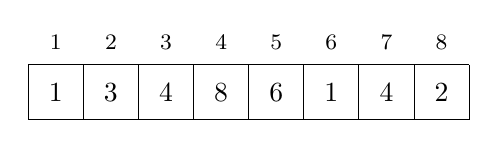
\begin{tikzpicture}[scale=0.7]
        \draw (0,0) grid (8,1);

        \node at (0.5,0.5) {$1$};
        \node at (1.5,0.5) {$3$};
        \node at (2.5,0.5) {$4$};
        \node at (3.5,0.5) {$8$};
        \node at (4.5,0.5) {$6$};
        \node at (5.5,0.5) {$1$};
        \node at (6.5,0.5) {$4$};
        \node at (7.5,0.5) {$2$};

        \footnotesize
        \node at (0.5,1.4) {$1$};
        \node at (1.5,1.4) {$2$};
        \node at (2.5,1.4) {$3$};
        \node at (3.5,1.4) {$4$};
        \node at (4.5,1.4) {$5$};
        \node at (5.5,1.4) {$6$};
        \node at (6.5,1.4) {$7$};
        \node at (7.5,1.4) {$8$};
    \end{tikzpicture}
\end{center}

El árbol binario indexado correspondiente es el siguiente:
\begin{center}
    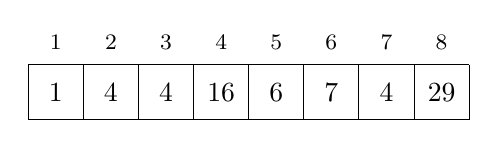
\begin{tikzpicture}[scale=0.7]
        \draw (0,0) grid (8,1);

        \node at (0.5,0.5) {$1$};
        \node at (1.5,0.5) {$4$};
        \node at (2.5,0.5) {$4$};
        \node at (3.5,0.5) {$16$};
        \node at (4.5,0.5) {$6$};
        \node at (5.5,0.5) {$7$};
        \node at (6.5,0.5) {$4$};
        \node at (7.5,0.5) {$29$};

        \footnotesize
        \node at (0.5,1.4) {$1$};
        \node at (1.5,1.4) {$2$};
        \node at (2.5,1.4) {$3$};
        \node at (3.5,1.4) {$4$};
        \node at (4.5,1.4) {$5$};
        \node at (5.5,1.4) {$6$};
        \node at (6.5,1.4) {$7$};
        \node at (7.5,1.4) {$8$};
    \end{tikzpicture}
\end{center}

La siguiente imagen muestra de manera más clara
cómo cada valor en el árbol binario indexado
corresponde a un rango en el arreglo original:

\begin{center}
    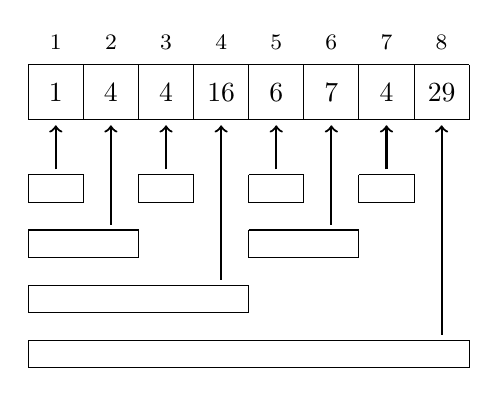
\begin{tikzpicture}[scale=0.7]
        \draw (0,0) grid (8,1);

        \node at (0.5,0.5) {$1$};
        \node at (1.5,0.5) {$4$};
        \node at (2.5,0.5) {$4$};
        \node at (3.5,0.5) {$16$};
        \node at (4.5,0.5) {$6$};
        \node at (5.5,0.5) {$7$};
        \node at (6.5,0.5) {$4$};
        \node at (7.5,0.5) {$29$};

        \footnotesize
        \node at (0.5,1.4) {$1$};
        \node at (1.5,1.4) {$2$};
        \node at (2.5,1.4) {$3$};
        \node at (3.5,1.4) {$4$};
        \node at (4.5,1.4) {$5$};
        \node at (5.5,1.4) {$6$};
        \node at (6.5,1.4) {$7$};
        \node at (7.5,1.4) {$8$};

        \draw[->,thick] (0.5,-0.9) -- (0.5,-0.1);
        \draw[->,thick] (2.5,-0.9) -- (2.5,-0.1);
        \draw[->,thick] (4.5,-0.9) -- (4.5,-0.1);
        \draw[->,thick] (6.5,-0.9) -- (6.5,-0.1);
        \draw[->,thick] (1.5,-1.9) -- (1.5,-0.1);
        \draw[->,thick] (5.5,-1.9) -- (5.5,-0.1);
        \draw[->,thick] (3.5,-2.9) -- (3.5,-0.1);
        \draw[->,thick] (7.5,-3.9) -- (7.5,-0.1);

        \draw (0,-1) -- (1,-1) -- (1,-1.5) -- (0,-1.5) -- (0,-1);
        \draw (2,-1) -- (3,-1) -- (3,-1.5) -- (2,-1.5) -- (2,-1);
        \draw (4,-1) -- (5,-1) -- (5,-1.5) -- (4,-1.5) -- (4,-1);
        \draw (6,-1) -- (7,-1) -- (7,-1.5) -- (6,-1.5) -- (6,-1);
        \draw (0,-2) -- (2,-2) -- (2,-2.5) -- (0,-2.5) -- (0,-2);
        \draw (4,-2) -- (6,-2) -- (6,-2.5) -- (4,-2.5) -- (4,-2);
        \draw (0,-3) -- (4,-3) -- (4,-3.5) -- (0,-3.5) -- (0,-3);
        \draw (0,-4) -- (8,-4) -- (8,-4.5) -- (0,-4.5) -- (0,-4);
    \end{tikzpicture}
\end{center}

Usando un árbol binario indexado,
cualquier valor de $\texttt{suma}_q(1,k)$
se puede calcular en $O(\log n)$,
porque un rango $[1,k]$ siempre se puede dividir en
$O(\log n)$ rangos cuyas sumas están almacenadas en el árbol.

Por ejemplo, el rango $[1,7]$ consta de
los siguientes rangos:
\begin{center}
    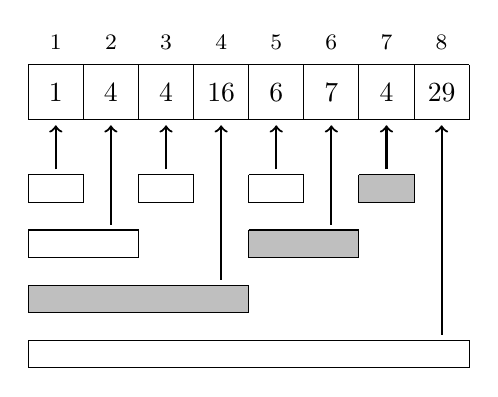
\begin{tikzpicture}[scale=0.7]
        \draw (0,0) grid (8,1);

        \node at (0.5,0.5) {$1$};
        \node at (1.5,0.5) {$4$};
        \node at (2.5,0.5) {$4$};
        \node at (3.5,0.5) {$16$};
        \node at (4.5,0.5) {$6$};
        \node at (5.5,0.5) {$7$};
        \node at (6.5,0.5) {$4$};
        \node at (7.5,0.5) {$29$};

        \footnotesize
        \node at (0.5,1.4) {$1$};
        \node at (1.5,1.4) {$2$};
        \node at (2.5,1.4) {$3$};
        \node at (3.5,1.4) {$4$};
        \node at (4.5,1.4) {$5$};
        \node at (5.5,1.4) {$6$};
        \node at (6.5,1.4) {$7$};
        \node at (7.5,1.4) {$8$};

        \draw[->,thick] (0.5,-0.9) -- (0.5,-0.1);
        \draw[->,thick] (2.5,-0.9) -- (2.5,-0.1);
        \draw[->,thick] (4.5,-0.9) -- (4.5,-0.1);
        \draw[->,thick] (6.5,-0.9) -- (6.5,-0.1);
        \draw[->,thick] (1.5,-1.9) -- (1.5,-0.1);
        \draw[->,thick] (5.5,-1.9) -- (5.5,-0.1);
        \draw[->,thick] (3.5,-2.9) -- (3.5,-0.1);
        \draw[->,thick] (7.5,-3.9) -- (7.5,-0.1);

        \draw (0,-1) -- (1,-1) -- (1,-1.5) -- (0,-1.5) -- (0,-1);
        \draw (2,-1) -- (3,-1) -- (3,-1.5) -- (2,-1.5) -- (2,-1);
        \draw (4,-1) -- (5,-1) -- (5,-1.5) -- (4,-1.5) -- (4,-1);
        \draw[fill=lightgray] (6,-1) -- (7,-1) -- (7,-1.5) -- (6,-1.5) -- (6,-1);
        \draw (0,-2) -- (2,-2) -- (2,-2.5) -- (0,-2.5) -- (0,-2);
        \draw[fill=lightgray] (4,-2) -- (6,-2) -- (6,-2.5) -- (4,-2.5) -- (4,-2);
        \draw[fill=lightgray] (0,-3) -- (4,-3) -- (4,-3.5) -- (0,-3.5) -- (0,-3);
        \draw (0,-4) -- (8,-4) -- (8,-4.5) -- (0,-4.5) -- (0,-4);
    \end{tikzpicture}
\end{center}
Por lo tanto, podemos calcular la suma correspondiente de la siguiente manera:
\[\texttt{suma}_q(1,7)=\texttt{suma}_q(1,4)+\texttt{suma}_q(5,6)+\texttt{suma}_q(7,7)=16+7+4=27\]

Para calcular el valor de $\texttt{suma}_q(a,b)$ donde $a>1$,
podemos usar el mismo truco que utilizamos con arreglos de sumas de prefijos:
\[ \texttt{suma}_q(a,b) = \texttt{suma}_q(1,b) - \texttt{suma}_q(1,a-1).\]
Dado que podemos calcular tanto $\texttt{suma}_q(1,b)$
como $\texttt{suma}_q(1,a-1)$ en $O(\log n)$,
la complejidad total del tiempo es $O(\log n)$.

Luego, después de actualizar un valor en el arreglo original,
varios valores en el árbol binario indexado
deben ser actualizados.
Por ejemplo, si el valor en la posición 3 cambia,
las sumas de los siguientes rangos cambian:
\begin{center}
    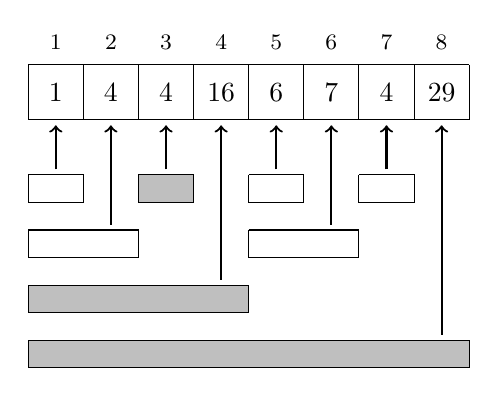
\begin{tikzpicture}[scale=0.7]
        \draw (0,0) grid (8,1);

        \node at (0.5,0.5) {$1$};
        \node at (1.5,0.5) {$4$};
        \node at (2.5,0.5) {$4$};
        \node at (3.5,0.5) {$16$};
        \node at (4.5,0.5) {$6$};
        \node at (5.5,0.5) {$7$};
        \node at (6.5,0.5) {$4$};
        \node at (7.5,0.5) {$29$};

        \footnotesize
        \node at (0.5,1.4) {$1$};
        \node at (1.5,1.4) {$2$};
        \node at (2.5,1.4) {$3$};
        \node at (3.5,1.4) {$4$};
        \node at (4.5,1.4) {$5$};
        \node at (5.5,1.4) {$6$};
        \node at (6.5,1.4) {$7$};
        \node at (7.5,1.4) {$8$};

        \draw[->,thick] (0.5,-0.9) -- (0.5,-0.1);
        \draw[->,thick] (2.5,-0.9) -- (2.5,-0.1);
        \draw[->,thick] (4.5,-0.9) -- (4.5,-0.1);
        \draw[->,thick] (6.5,-0.9) -- (6.5,-0.1);
        \draw[->,thick] (1.5,-1.9) -- (1.5,-0.1);
        \draw[->,thick] (5.5,-1.9) -- (5.5,-0.1);
        \draw[->,thick] (3.5,-2.9) -- (3.5,-0.1);
        \draw[->,thick] (7.5,-3.9) -- (7.5,-0.1);

        \draw (0,-1) -- (1,-1) -- (1,-1.5) -- (0,-1.5) -- (0,-1);
        \draw[fill=lightgray] (2,-1) -- (3,-1) -- (3,-1.5) -- (2,-1.5) -- (2,-1);
        \draw (4,-1) -- (5,-1) -- (5,-1.5) -- (4,-1.5) -- (4,-1);
        \draw (6,-1) -- (7,-1) -- (7,-1.5) -- (6,-1.5) -- (6,-1);
        \draw (0,-2) -- (2,-2) -- (2,-2.5) -- (0,-2.5) -- (0,-2);
        \draw (4,-2) -- (6,-2) -- (6,-2.5) -- (4,-2.5) -- (4,-2);
        \draw[fill=lightgray] (0,-3) -- (4,-3) -- (4,-3.5) -- (0,-3.5) -- (0,-3);
        \draw[fill=lightgray] (0,-4) -- (8,-4) -- (8,-4.5) -- (0,-4.5) -- (0,-4);
    \end{tikzpicture}
\end{center}

Dado que cada elemento del arreglo pertenece a $O(\log n)$
rangos en el árbol binario indexado,
basta con actualizar $O(\log n)$ valores en el árbol.

\subsubsection{Implementación}

Las operaciones de un árbol binario indexado pueden ser
implementadas de manera eficiente usando operaciones de bits.
El hecho clave necesario es que podemos
calcular cualquier valor de $p(k)$ usando la siguiente fórmula:
\[p(k) = k \& (-k)\]

La siguiente función calcula el valor de $\texttt{suma}_q(1,k)$:
\begin{lstlisting}
int suma(int k) {
    int s = 0;
    while (k >= 1) {
        s += árbol[k];
        k -= k & -k;
    }
    return s;
}
\end{lstlisting}

\newpage
La siguiente función aumenta el
valor del arreglo en la posición $k$ por $x$
($x$ puede ser positivo o negativo):

\begin{lstlisting}
void agregar(int k, int x) {
    while (k <= n) {
        árbol[k] += x;
        k += k & -k;
    }
}
\end{lstlisting}

La complejidad temporal de ambas funciones es
$O(\log n)$, porque las funciones acceden a $O(\log n)$
valores en el árbol binario indexado, y cada movimiento
a la siguiente posición toma $O(1)$.

\section{Árbol de segmentos}

\index{árbol de segmentos}

Un \key{árbol de segmentos}\footnote{La implementación de abajo hacia arriba en este capítulo corresponde
    a la que aparece en \cite{sta06}. Estructuras similares se utilizaron
    a finales de la década de 1970 para resolver problemas geométricos \cite{ben80}.} es una estructura de datos
que soporta dos operaciones:
procesar una consulta de rango y
actualizar un valor del arreglo.
Los árboles de segmentos pueden soportar
consultas de suma, consultas de mínimo y máximo, y muchas otras
consultas de modo que ambas operaciones funcionen en $O(\log n)$.

En comparación con un árbol binario indexado,
la ventaja de un árbol de segmentos es que es
una estructura de datos más general.
Mientras que los árboles binarios indexados solo admiten
consultas de suma,\footnote{De hecho, utilizando \emph{dos} árboles
    binarios indexados es posible soportar consultas de mínimo \cite{dim15},
    pero esto es más complicado que usar un árbol de segmentos.}
los árboles de segmentos también admiten otras consultas.
Por otro lado, un árbol de segmentos requiere más
memoria y es un poco más difícil de implementar.

\subsubsection{Estructura}

Un árbol de segmentos es un árbol binario
tal que los nodos en el nivel inferior del árbol
corresponden a los elementos del arreglo,
y los otros nodos
contienen información necesaria para procesar consultas de rango.

En esta sección, asumimos que el tamaño
del arreglo es una potencia de dos y se utiliza indexación basada en cero,
porque es conveniente construir
un árbol de segmentos para tal arreglo.
Si el tamaño del arreglo no es una potencia de dos,
siempre podemos agregar elementos adicionales.

Primero discutiremos árboles de segmentos que admiten consultas de suma.
Como ejemplo, considera el siguiente arreglo:
\begin{center}
    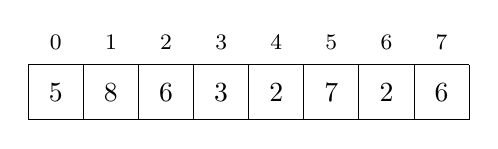
\begin{tikzpicture}[scale=0.7]
        \draw (0,0) grid (8,1);

        \node at (0.5,0.5) {$5$};
        \node at (1.5,0.5) {$8$};
        \node at (2.5,0.5) {$6$};
        \node at (3.5,0.5) {$3$};
        \node at (4.5,0.5) {$2$};
        \node at (5.5,0.5) {$7$};
        \node at (6.5,0.5) {$2$};
        \node at (7.5,0.5) {$6$};

        \footnotesize
        \node at (0.5,1.4) {$0$};
        \node at (1.5,1.4) {$1$};
        \node at (2.5,1.4) {$2$};
        \node at (3.5,1.4) {$3$};
        \node at (4.5,1.4) {$4$};
        \node at (5.5,1.4) {$5$};
        \node at (6.5,1.4) {$6$};
        \node at (7.5,1.4) {$7$};
    \end{tikzpicture}
\end{center}

\newpage
El árbol de segmentos correspondiente es el siguiente:
\begin{center}
    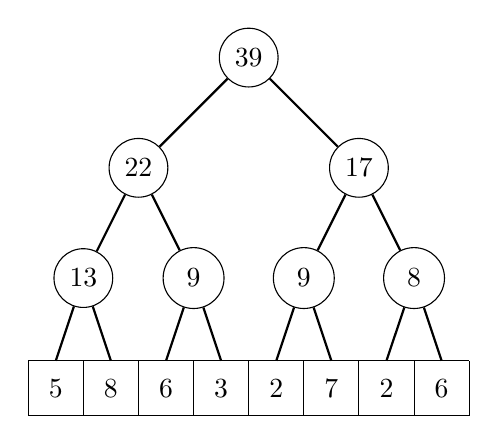
\begin{tikzpicture}[scale=0.7]
        \draw (0,0) grid (8,1);

        \node[anchor=center] at (0.5, 0.5) {5};
        \node[anchor=center] at (1.5, 0.5) {8};
        \node[anchor=center] at (2.5, 0.5) {6};
        \node[anchor=center] at (3.5, 0.5) {3};
        \node[anchor=center] at (4.5, 0.5) {2};
        \node[anchor=center] at (5.5, 0.5) {7};
        \node[anchor=center] at (6.5, 0.5) {2};
        \node[anchor=center] at (7.5, 0.5) {6};

        \node[draw, circle] (a) at (1,2.5) {13};
        \path[draw,thick,-] (a) -- (0.5,1);
        \path[draw,thick,-] (a) -- (1.5,1);
        \node[draw, circle,minimum size=22pt] (b) at (3,2.5) {9};
        \path[draw,thick,-] (b) -- (2.5,1);
        \path[draw,thick,-] (b) -- (3.5,1);
        \node[draw, circle,minimum size=22pt] (c) at (5,2.5) {9};
        \path[draw,thick,-] (c) -- (4.5,1);
        \path[draw,thick,-] (c) -- (5.5,1);
        \node[draw, circle,minimum size=22pt] (d) at (7,2.5) {8};
        \path[draw,thick,-] (d) -- (6.5,1);
        \path[draw,thick,-] (d) -- (7.5,1);

        \node[draw, circle] (i) at (2,4.5) {22};
        \path[draw,thick,-] (i) -- (a);
        \path[draw,thick,-] (i) -- (b);
        \node[draw, circle] (j) at (6,4.5) {17};
        \path[draw,thick,-] (j) -- (c);
        \path[draw,thick,-] (j) -- (d);

        \node[draw, circle] (m) at (4,6.5) {39};
        \path[draw,thick,-] (m) -- (i);
        \path[draw,thick,-] (m) -- (j);
    \end{tikzpicture}
\end{center}

Cada nodo interno del árbol
corresponde a un rango de arreglo
cuyo tamaño es una potencia de dos.
En el árbol anterior, el valor de cada nodo
es la suma de los valores del arreglo correspondiente,
y se puede calcular como la suma de
los valores de su nodo hijo izquierdo y derecho.

Resulta que cualquier rango $[a,b]$
puede dividirse en $O(\log n)$ rangos
cuyos valores se almacenan en nodos del árbol.
Por ejemplo, considera el rango [2,7]:
\begin{center}
    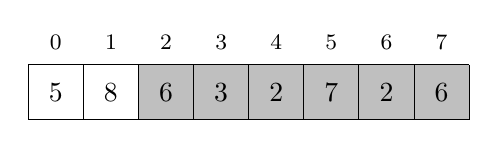
\begin{tikzpicture}[scale=0.7]
        \fill[color=gray!50] (2,0) rectangle (8,1);
        \draw (0,0) grid (8,1);

        \node[anchor=center] at (0.5, 0.5) {5};
        \node[anchor=center] at (1.5, 0.5) {8};
        \node[anchor=center] at (2.5, 0.5) {6};
        \node[anchor=center] at (3.5, 0.5) {3};
        \node[anchor=center] at (4.5, 0.5) {2};
        \node[anchor=center] at (5.5, 0.5) {7};
        \node[anchor=center] at (6.5, 0.5) {2};
        \node[anchor=center] at (7.5, 0.5) {6};

        \footnotesize
        \node at (0.5,1.4) {$0$};
        \node at (1.5,1.4) {$1$};
        \node at (2.5,1.4) {$2$};
        \node at (3.5,1.4) {$3$};
        \node at (4.5,1.4) {$4$};
        \node at (5.5,1.4) {$5$};
        \node at (6.5,1.4) {$6$};
        \node at (7.5,1.4) {$7$};
    \end{tikzpicture}
\end{center}
Aquí $\texttt{suma}_q(2,7)=6+3+2+7+2+6=26$.
En este caso, los siguientes dos nodos del árbol
corresponden al rango:
\begin{center}
    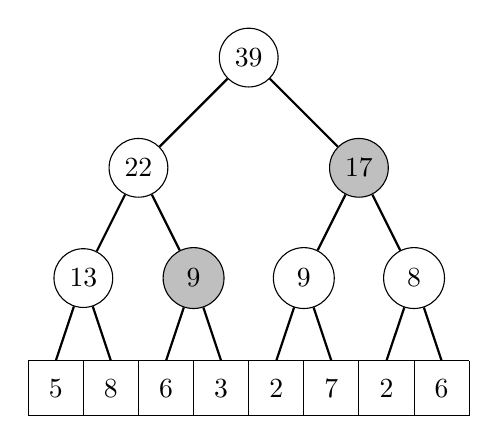
\begin{tikzpicture}[scale=0.7]
        \draw (0,0) grid (8,1);

        \node[anchor=center] at (0.5, 0.5) {5};
        \node[anchor=center] at (1.5, 0.5) {8};
        \node[anchor=center] at (2.5, 0.5) {6};
        \node[anchor=center] at (3.5, 0.5) {3};
        \node[anchor=center] at (4.5, 0.5) {2};
        \node[anchor=center] at (5.5, 0.5) {7};
        \node[anchor=center] at (6.5, 0.5) {2};
        \node[anchor=center] at (7.5, 0.5) {6};

        \node[draw, circle] (a) at (1,2.5) {13};
        \path[draw,thick,-] (a) -- (0.5,1);
        \path[draw,thick,-] (a) -- (1.5,1);
        \node[draw, circle,fill=gray!50,minimum size=22pt] (b) at (3,2.5) {9};
        \path[draw,thick,-] (b) -- (2.5,1);
        \path[draw,thick,-] (b) -- (3.5,1);
        \node[draw, circle,minimum size=22pt] (c) at (5,2.5) {9};
        \path[draw,thick,-] (c) -- (4.5,1);
        \path[draw,thick,-] (c) -- (5.5,1);
        \node[draw, circle,minimum size=22pt] (d) at (7,2.5) {8};
        \path[draw,thick,-] (d) -- (6.5,1);
        \path[draw,thick,-] (d) -- (7.5,1);

        \node[draw, circle] (i) at (2,4.5) {22};
        \path[draw,thick,-] (i) -- (a);
        \path[draw,thick,-] (i) -- (b);
        \node[draw, circle,fill=gray!50] (j) at (6,4.5) {17};
        \path[draw,thick,-] (j) -- (c);
        \path[draw,thick,-] (j) -- (d);

        \node[draw, circle] (m) at (4,6.5) {39};
        \path[draw,thick,-] (m) -- (i);
        \path[draw,thick,-] (m) -- (j);
    \end{tikzpicture}
\end{center}
Por lo tanto, otra forma de calcular la suma es $9+17=26$.

Cuando se calcula la suma utilizando nodos
ubicados lo más alto posible en el árbol,
se necesitan como máximo dos nodos en cada nivel
del árbol.
Por lo tanto, el número total de nodos
es $O(\log n)$.

Después de una actualización del arreglo,
debemos actualizar todos los nodos
cuyos valores dependan del valor actualizado.
Esto se puede hacer recorriendo el camino
desde el elemento de matriz actualizado hasta el nodo superior
y actualizando los nodos a lo largo del camino.

\newpage
La siguiente imagen muestra qué nodos del árbol
cambian si modificamos el valor 7 del arreglo:

\begin{center}
    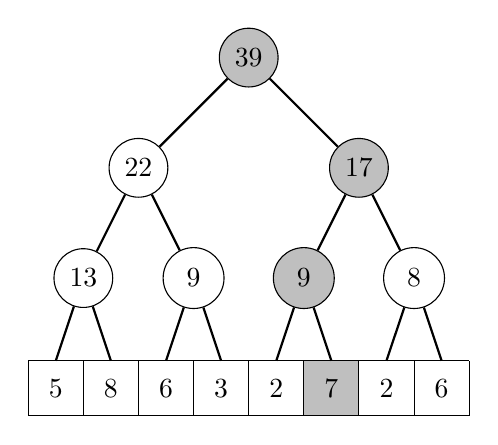
\begin{tikzpicture}[scale=0.7]
        \fill[color=gray!50] (5,0) rectangle (6,1);
        \draw (0,0) grid (8,1);

        \node[anchor=center] at (0.5, 0.5) {5};
        \node[anchor=center] at (1.5, 0.5) {8};
        \node[anchor=center] at (2.5, 0.5) {6};
        \node[anchor=center] at (3.5, 0.5) {3};
        \node[anchor=center] at (4.5, 0.5) {2};
        \node[anchor=center] at (5.5, 0.5) {7};
        \node[anchor=center] at (6.5, 0.5) {2};
        \node[anchor=center] at (7.5, 0.5) {6};

        \node[draw, circle] (a) at (1,2.5) {13};
        \path[draw,thick,-] (a) -- (0.5,1);
        \path[draw,thick,-] (a) -- (1.5,1);
        \node[draw, circle,minimum size=22pt] (b) at (3,2.5) {9};
        \path[draw,thick,-] (b) -- (2.5,1);
        \path[draw,thick,-] (b) -- (3.5,1);
        \node[draw, circle,minimum size=22pt,fill=gray!50] (c) at (5,2.5) {9};
        \path[draw,thick,-] (c) -- (4.5,1);
        \path[draw,thick,-] (c) -- (5.5,1);
        \node[draw, circle,minimum size=22pt] (d) at (7,2.5) {8};
        \path[draw,thick,-] (d) -- (6.5,1);
        \path[draw,thick,-] (d) -- (7.5,1);

        \node[draw, circle] (i) at (2,4.5) {22};
        \path[draw,thick,-] (i) -- (a);
        \path[draw,thick,-] (i) -- (b);
        \node[draw, circle,fill=gray!50] (j) at (6,4.5) {17};
        \path[draw,thick,-] (j) -- (c);
        \path[draw,thick,-] (j) -- (d);

        \node[draw, circle,fill=gray!50] (m) at (4,6.5) {39};
        \path[draw,thick,-] (m) -- (i);
        \path[draw,thick,-] (m) -- (j);
    \end{tikzpicture}
\end{center}

El camino de abajo hacia arriba
siempre consta de $O(\log n)$ nodos,
por lo que cada actualización cambia $O(\log n)$ nodos en el árbol.

\subsubsection{Implementación}

Similarmente al árbol binario indexado, el árbol de segmentos
se almacena en un arreglo.

Almacenamos un árbol de segmentos como un arreglo
de $2n$ elementos, donde $n$ es el tamaño del
arreglo original y a la vez una potencia de dos.
Los nodos del árbol se almacenan de arriba hacia abajo:
$\texttt{arbol}[1]$ es el nodo superior (la raíz),
$\texttt{arbol}[2]$ y $\texttt{arbol}[3]$
son sus hijos, y así sucesivamente.
Finalmente, los valores desde $\texttt{arbol}[n]$
hasta $\texttt{arbol}[2n-1]$ corresponden a
los valores del arreglo original
en el nivel inferior del árbol.

Por ejemplo, el siguiente árbol de segmentos:
\begin{center}
    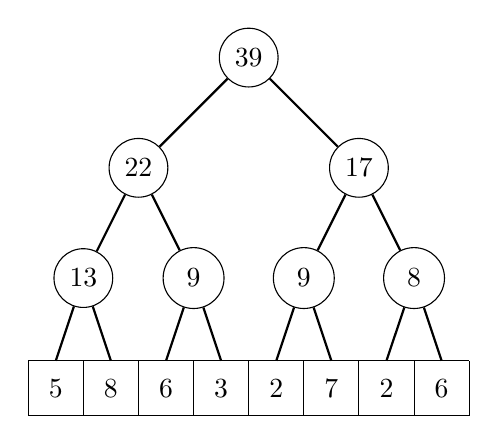
\begin{tikzpicture}[scale=0.7]
        \draw (0,0) grid (8,1);

        \node[anchor=center] at (0.5, 0.5) {5};
        \node[anchor=center] at (1.5, 0.5) {8};
        \node[anchor=center] at (2.5, 0.5) {6};
        \node[anchor=center] at (3.5, 0.5) {3};
        \node[anchor=center] at (4.5, 0.5) {2};
        \node[anchor=center] at (5.5, 0.5) {7};
        \node[anchor=center] at (6.5, 0.5) {2};
        \node[anchor=center] at (7.5, 0.5) {6};

        \node[draw, circle] (a) at (1,2.5) {13};
        \path[draw,thick,-] (a) -- (0.5,1);
        \path[draw,thick,-] (a) -- (1.5,1);
        \node[draw, circle,minimum size=22pt] (b) at (3,2.5) {9};
        \path[draw,thick,-] (b) -- (2.5,1);
        \path[draw,thick,-] (b) -- (3.5,1);
        \node[draw, circle,minimum size=22pt] (c) at (5,2.5) {9};
        \path[draw,thick,-] (c) -- (4.5,1);
        \path[draw,thick,-] (c) -- (5.5,1);
        \node[draw, circle,minimum size=22pt] (d) at (7,2.5) {8};
        \path[draw,thick,-] (d) -- (6.5,1);
        \path[draw,thick,-] (d) -- (7.5,1);

        \node[draw, circle] (i) at (2,4.5) {22};
        \path[draw,thick,-] (i) -- (a);
        \path[draw,thick,-] (i) -- (b);
        \node[draw, circle] (j) at (6,4.5) {17};
        \path[draw,thick,-] (j) -- (c);
        \path[draw,thick,-] (j) -- (d);

        \node[draw, circle] (m) at (4,6.5) {39};
        \path[draw,thick,-] (m) -- (i);
        \path[draw,thick,-] (m) -- (j);
    \end{tikzpicture}
\end{center}

se almacena de la siguiente manera:
\begin{center}
    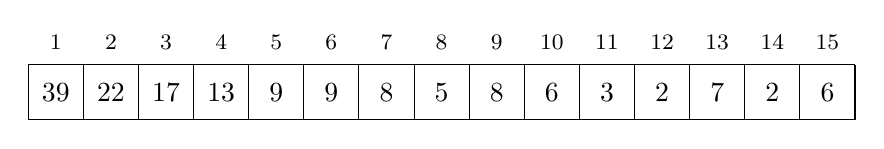
\begin{tikzpicture}[scale=0.7]
        \draw (0,0) grid (15,1);

        \node at (0.5,0.5) {$39$};
        \node at (1.5,0.5) {$22$};
        \node at (2.5,0.5) {$17$};
        \node at (3.5,0.5) {$13$};
        \node at (4.5,0.5) {$9$};
        \node at (5.5,0.5) {$9$};
        \node at (6.5,0.5) {$8$};
        \node at (7.5,0.5) {$5$};
        \node at (8.5,0.5) {$8$};
        \node at (9.5,0.5) {$6$};
        \node at (10.5,0.5) {$3$};
        \node at (11.5,0.5) {$2$};
        \node at (12.5,0.5) {$7$};
        \node at (13.5,0.5) {$2$};
        \node at (14.5,0.5) {$6$};

        \footnotesize
        \node at (0.5,1.4) {$1$};
        \node at (1.5,1.4) {$2$};
        \node at (2.5,1.4) {$3$};
        \node at (3.5,1.4) {$4$};
        \node at (4.5,1.4) {$5$};
        \node at (5.5,1.4) {$6$};
        \node at (6.5,1.4) {$7$};
        \node at (7.5,1.4) {$8$};
        \node at (8.5,1.4) {$9$};
        \node at (9.5,1.4) {$10$};
        \node at (10.5,1.4) {$11$};
        \node at (11.5,1.4) {$12$};
        \node at (12.5,1.4) {$13$};
        \node at (13.5,1.4) {$14$};
        \node at (14.5,1.4) {$15$};
    \end{tikzpicture}
\end{center}

\newpage
La siguiente función
calcula el valor de $\texttt{suma}_q(a,b)$:
\begin{lstlisting}
int suma(int a, int b) {
    a += n; b += n;
    int s = 0;
    while (a <= b) {
        if (a % 2 == 1) s += árbol[a++];
        if (b % 2 == 0) s += árbol[b--];
        a /= 2; b /= 2;
    }
    return s;
}
\end{lstlisting}
La función mantiene un rango
que inicialmente es $[a+n,b+n]$.
Luego, en cada paso, el rango se mueve
un nivel más alto en el árbol,
y antes de eso, los valores de los nodos que no
pertenecen al rango superior se añaden a la suma.

La siguiente función incrementa el valor del arreglo
en la posición $k$ por $x$:
\begin{lstlisting}
void agregar(int k, int x) {
    k += n;
    árbol[k] += x;
    for (k /= 2; k >= 1; k /= 2) {
        árbol[k] = árbol[2 * k] + árbol[2 * k + 1];
    }
}
\end{lstlisting}
Primero, la función actualiza el valor
en el nivel inferior del árbol.
Después de esto, la función actualiza los valores de todos
los nodos internos del árbol, hasta que llega
al nodo superior del árbol.

Ambas funciones trabajan
en $O(\log n)$, porque un árbol de segmentos
de $n$ elementos consiste en $O(\log n)$ niveles,
y las funciones se mueven un nivel más alto
en el árbol en cada paso.

\subsubsection{Otras consultas}

Los árboles de segmentos pueden admitir todas las consultas de rango
donde es posible dividir un rango en dos partes,
calcular la respuesta por separado para ambas partes
y luego combinar eficientemente las respuestas.
Ejemplos de tales consultas son
mínimo (\texttt{min}) y máximo (\texttt{max}),
máximo común divisor (\texttt{gcd}) y mínimo común múltiplo (\texttt{lcm}),
y operaciones lógicas como and (\texttt{\&}), or (\texttt{\textbar}) y xor (\texttt{\^{}}).

\newpage
Por ejemplo, el siguiente árbol de segmentos
admite consultas de mínimos:

\begin{center}
    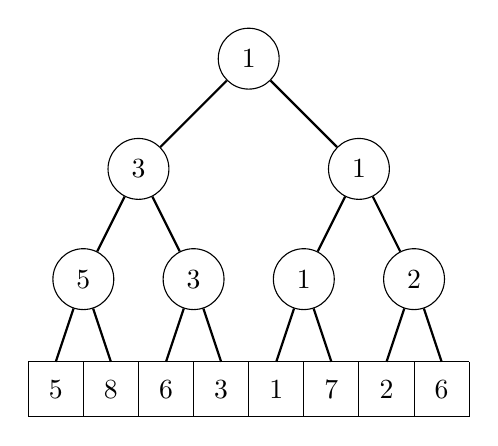
\begin{tikzpicture}[scale=0.7]
        \draw (0,0) grid (8,1);

        \node[anchor=center] at (0.5, 0.5) {5};
        \node[anchor=center] at (1.5, 0.5) {8};
        \node[anchor=center] at (2.5, 0.5) {6};
        \node[anchor=center] at (3.5, 0.5) {3};
        \node[anchor=center] at (4.5, 0.5) {1};
        \node[anchor=center] at (5.5, 0.5) {7};
        \node[anchor=center] at (6.5, 0.5) {2};
        \node[anchor=center] at (7.5, 0.5) {6};

        \node[draw, circle,minimum size=22pt] (a) at (1,2.5) {5};
        \path[draw,thick,-] (a) -- (0.5,1);
        \path[draw,thick,-] (a) -- (1.5,1);
        \node[draw, circle,minimum size=22pt] (b) at (3,2.5) {3};
        \path[draw,thick,-] (b) -- (2.5,1);
        \path[draw,thick,-] (b) -- (3.5,1);
        \node[draw, circle,minimum size=22pt] (c) at (5,2.5) {1};
        \path[draw,thick,-] (c) -- (4.5,1);
        \path[draw,thick,-] (c) -- (5.5,1);
        \node[draw, circle,minimum size=22pt] (d) at (7,2.5) {2};
        \path[draw,thick,-] (d) -- (6.5,1);
        \path[draw,thick,-] (d) -- (7.5,1);

        \node[draw, circle,minimum size=22pt] (i) at (2,4.5) {3};
        \path[draw,thick,-] (i) -- (a);
        \path[draw,thick,-] (i) -- (b);
        \node[draw, circle,minimum size=22pt] (j) at (6,4.5) {1};
        \path[draw,thick,-] (j) -- (c);
        \path[draw,thick,-] (j) -- (d);

        \node[draw, circle,minimum size=22pt] (m) at (4,6.5) {1};
        \path[draw,thick,-] (m) -- (i);
        \path[draw,thick,-] (m) -- (j);
    \end{tikzpicture}
\end{center}

En este caso, cada nodo del árbol contiene
el valor más pequeño en el rango correspondiente
del arreglo.
El nodo superior del árbol contiene el valor más pequeño
en todo el arreglo.
Las operaciones se pueden implementar como antes,
pero en lugar de sumas, se calculan los mínimos.

La estructura de un árbol de segmentos también nos permite
usar búsqueda binaria para localizar elementos del arreglo.
Por ejemplo, si el árbol admite consultas de mínimo,
podemos encontrar la posición de un elemento
con el valor más pequeño en $O(\log n)$.

Por ejemplo, en el árbol anterior, un
elemento con el valor más pequeño 1 se puede encontrar
recorriendo un camino hacia abajo desde el nodo superior:

\begin{center}
    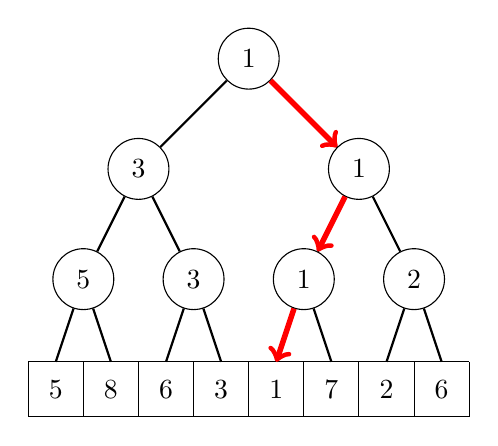
\begin{tikzpicture}[scale=0.7]
        \draw (0,0) grid (8,1);

        \node[anchor=center] at (0.5, 0.5) {5};
        \node[anchor=center] at (1.5, 0.5) {8};
        \node[anchor=center] at (2.5, 0.5) {6};
        \node[anchor=center] at (3.5, 0.5) {3};
        \node[anchor=center] at (4.5, 0.5) {1};
        \node[anchor=center] at (5.5, 0.5) {7};
        \node[anchor=center] at (6.5, 0.5) {2};
        \node[anchor=center] at (7.5, 0.5) {6};

        \node[draw, circle,minimum size=22pt] (a) at (1,2.5) {5};
        \path[draw,thick,-] (a) -- (0.5,1);
        \path[draw,thick,-] (a) -- (1.5,1);
        \node[draw, circle,minimum size=22pt] (b) at (3,2.5) {3};
        \path[draw,thick,-] (b) -- (2.5,1);
        \path[draw,thick,-] (b) -- (3.5,1);
        \node[draw, circle,minimum size=22pt] (c) at (5,2.5) {1};
        \path[draw,thick,-] (c) -- (4.5,1);
        \path[draw,thick,-] (c) -- (5.5,1);
        \node[draw, circle,minimum size=22pt] (d) at (7,2.5) {2};
        \path[draw,thick,-] (d) -- (6.5,1);
        \path[draw,thick,-] (d) -- (7.5,1);

        \node[draw, circle,minimum size=22pt] (i) at (2,4.5) {3};
        \path[draw,thick,-] (i) -- (a);
        \path[draw,thick,-] (i) -- (b);
        \node[draw, circle,minimum size=22pt] (j) at (6,4.5) {1};
        \path[draw,thick,-] (j) -- (c);
        \path[draw,thick,-] (j) -- (d);

        \node[draw, circle,minimum size=22pt] (m) at (4,6.5) {1};
        \path[draw,thick,-] (m) -- (i);
        \path[draw,thick,-] (m) -- (j);

        \path[draw=red,thick,->,line width=2pt] (m) -- (j);
        \path[draw=red,thick,->,line width=2pt] (j) -- (c);
        \path[draw=red,thick,->,line width=2pt] (c) -- (4.5,1);
    \end{tikzpicture}
\end{center}

\section{Técnicas adicionales}

\subsubsection{Compresión de índices}

Una limitación en las estructuras de datos que
se basan en un arreglo es que
los elementos se indexan usando
enteros consecutivos.
Se presentan dificultades cuando se necesitan índices grandes.
Por ejemplo, si deseamos usar el índice $10^9$,
el arreglo debería contener $10^9$
elementos, lo que requeriría demasiada memoria.

\index{compresión de índices}

Sin embargo, a menudo podemos eludir esta limitación
utilizando \key{compresión de índices},
donde los índices originales son reemplazados
con índices $1,2,3,$ etc.
Esto se puede hacer si conocemos todos los índices
necesarios durante el algoritmo de antemano.

La idea es reemplazar cada índice original $x$
con $c(x)$ donde $c$ es una función que
comprime los índices.
Requerimos que el orden de los índices
no cambie, así que si $a<b$, entonces $c(a)<c(b)$.
Esto nos permite realizar consultas convenientemente
incluso si los índices están comprimidos.

Por ejemplo, si los índices originales son
$555$, $10^9$ y $8$, los nuevos índices son:

\[
    \begin{array}{lcl}
        c(8)    & = & 1 \\
        c(555)  & = & 2 \\
        c(10^9) & = & 3 \\
    \end{array}
\]

\subsubsection{Actualizaciones de rango}

Hasta ahora, hemos implementado estructuras de datos
que admiten consultas de rangos y actualizaciones
por índices. Consideremos ahora una situación opuesta,
donde debemos actualizar rangos y consultar índices.
Nos enfocaremos en una operación que aumenta todos
los elementos en un rango $[a,b]$ por $x$.

\index{arreglo de diferencias}

Sorprendentemente, podemos usar las estructuras de datos
presentadas en este capítulo también en esta situación.
Para hacer esto, construimos un \key{arreglo de diferencias}
cuyos valores indican
las diferencias entre valores consecutivos
en el arreglo original.
Por lo tanto, el arreglo original es el
arreglo de sumas de prefijos del
arreglo de diferencias.
Por ejemplo, considera el siguiente arreglo:

\begin{center}
    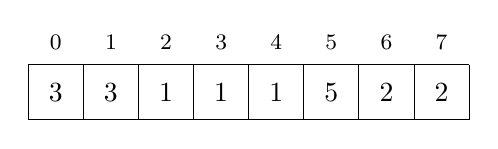
\begin{tikzpicture}[scale=0.7]
        \draw (0,0) grid (8,1);

        \node at (0.5,0.5) {$3$};
        \node at (1.5,0.5) {$3$};
        \node at (2.5,0.5) {$1$};
        \node at (3.5,0.5) {$1$};
        \node at (4.5,0.5) {$1$};
        \node at (5.5,0.5) {$5$};
        \node at (6.5,0.5) {$2$};
        \node at (7.5,0.5) {$2$};


        \footnotesize
        \node at (0.5,1.4) {$0$};
        \node at (1.5,1.4) {$1$};
        \node at (2.5,1.4) {$2$};
        \node at (3.5,1.4) {$3$};
        \node at (4.5,1.4) {$4$};
        \node at (5.5,1.4) {$5$};
        \node at (6.5,1.4) {$6$};
        \node at (7.5,1.4) {$7$};
    \end{tikzpicture}
\end{center}

El arreglo de diferencias para el arreglo anterior es el siguiente:
\begin{center}
    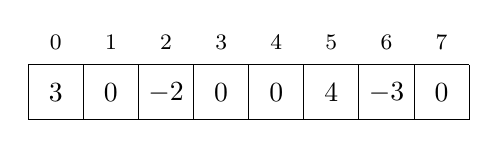
\begin{tikzpicture}[scale=0.7]
        \draw (0,0) grid (8,1);

        \node at (0.5,0.5) {$3$};
        \node at (1.5,0.5) {$0$};
        \node at (2.5,0.5) {$-2$};
        \node at (3.5,0.5) {$0$};
        \node at (4.5,0.5) {$0$};
        \node at (5.5,0.5) {$4$};
        \node at (6.5,0.5) {$-3$};
        \node at (7.5,0.5) {$0$};


        \footnotesize
        \node at (0.5,1.4) {$0$};
        \node at (1.5,1.4) {$1$};
        \node at (2.5,1.4) {$2$};
        \node at (3.5,1.4) {$3$};
        \node at (4.5,1.4) {$4$};
        \node at (5.5,1.4) {$5$};
        \node at (6.5,1.4) {$6$};
        \node at (7.5,1.4) {$7$};
    \end{tikzpicture}
\end{center}

Por ejemplo, el valor 2 en la posición 6 en el arreglo original
corresponde a la suma $3-2+4-3=2$ en el arreglo de diferencias.

La ventaja del arreglo de diferencias es
que podemos actualizar un rango
en el arreglo original cambiando solo
dos elementos en el arreglo de diferencias.
Por ejemplo, si queremos
aumentar el rango $[1, 4]$ por 5,
basta con aumentar el
valor del arreglo de diferencias en la posición 1 por 5
y disminuir el valor en la posición 5 por 5.
El resultado es el siguiente:

\begin{center}
    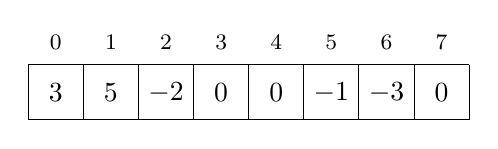
\begin{tikzpicture}[scale=0.7]
        \draw (0,0) grid (8,1);

        \node at (0.5,0.5) {$3$};
        \node at (1.5,0.5) {$5$};
        \node at (2.5,0.5) {$-2$};
        \node at (3.5,0.5) {$0$};
        \node at (4.5,0.5) {$0$};
        \node at (5.5,0.5) {$-1$};
        \node at (6.5,0.5) {$-3$};
        \node at (7.5,0.5) {$0$};

        \footnotesize
        \node at (0.5,1.4) {$0$};
        \node at (1.5,1.4) {$1$};
        \node at (2.5,1.4) {$2$};
        \node at (3.5,1.4) {$3$};
        \node at (4.5,1.4) {$4$};
        \node at (5.5,1.4) {$5$};
        \node at (6.5,1.4) {$6$};
        \node at (7.5,1.4) {$7$};
    \end{tikzpicture}
\end{center}

Más generalmente, para aumentar los valores
en el rango $[a,b]$ por $x$,
aumentamos el valor en la posición $a$ por $x$
y disminuimos el valor en la posición $b+1$ por $x$.
Por lo tanto, solo es necesario actualizar valores individuales
y procesar consultas de suma,
así que podemos usar un árbol binario indexado o un árbol de segmentos.

Un problema más difícil es admitir tanto
consultas de rango como actualizaciones de rango.
En el Capítulo 28 veremos que incluso esto es posible.




